\documentclass[12pt, twoside]{article}
\usepackage[letterpaper, margin=1in, headsep=0.5in]{geometry}
\usepackage[english]{babel}
\usepackage[utf8]{inputenc}
\usepackage{amsmath}
\usepackage{amsfonts}
\usepackage{amssymb}
\usepackage{tikz}
\usetikzlibrary{quotes, angles}
\usepackage{graphicx}
%\usepackage{pgfplots}
%\pgfplotsset{width=10cm,compat=1.9}
%\usepgfplotslibrary{statistics}
%\usepackage{pgfplotstable}
%\usepackage{tkz-fct}
%\usepackage{venndiagram}
\usepackage{enumitem}
\usepackage{multicol}


\usepackage{fancyhdr}
\pagestyle{fancy}
\fancyhf{}
\fancyhead[LE]{\thepage}
\fancyhead[RO]{%\thepage \\
    Name: \hspace{4cm} \,\\}
\fancyhead[LO]{BECA / Dr. Huson / Geometry 10th Grade\\* Unit 11: Algebra II introduction \\ 12 May 2020}

\renewcommand{\headrulewidth}{0pt}

\begin{document}
\subsubsection*{11.6 Problem set: Exact values of standard trigonometry ratios}

\begin{enumerate}

  \item A right $\triangle ABC$ is shown with side lengths 1, $\sqrt{3}$, and 2, as marked. \\[0.2cm]
  Identify each true statement%\vspace{0.5cm}
  \begin{multicols}{2}
    \begin{enumerate}[itemsep=0.4cm]
      \item[$\square$ (a)] $\displaystyle 1^2 + (\sqrt{3})^2 = 2^2$
      \item[$\square$ (b)] $\displaystyle \cos A=\frac{1}{2}$
      \item[$\square$ (c)] $\displaystyle \sin B= \frac{\sqrt{3}}{2}$
      \item[$\square$ (d)] $m\angle A = 60^\circ$
      \item[$\square$ (e)] $\displaystyle \cos B= \frac{\sqrt{3}}{2}$
      \item[$\square$ (f)] $m\angle A = 2 \times m\angle B$
      \end{enumerate}
        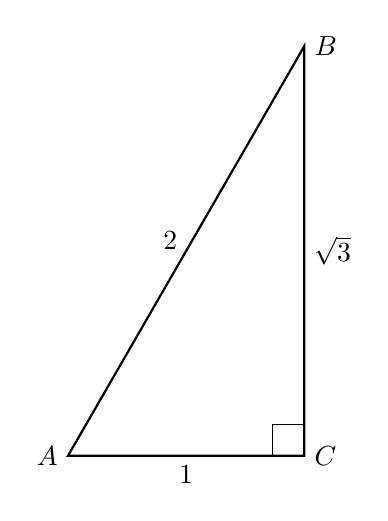
\begin{tikzpicture}[scale=1]
          \draw [thick]
          (0,0)node[left]{$A$}--
          (3,0)node[ right]{$C$}--
          (3,5.2)node[right]{$B$}--cycle;
          \draw (3,0)++(-0.4,0)--++(0,0.4)--+(0.4,0);
          \node at (1.5,0)[below]{$1$};
          \node at (3,2.6)[right]{$\sqrt{3}$};
          \node at (1.3,2.5)[above]{$2$};
        \end{tikzpicture}
    \end{multicols} %\vspace{0.5cm}

  \item Two similar, right isosceles triangles $\triangle HAT \sim \triangle CAB$ have a scale factor $k= 3$. Angles $\angle H$ and $\angle C$ measure $90^\circ$ and $HA=HT=1$, as shown.
  \begin{multicols}{2}
    \begin{enumerate}[itemsep=0.4cm]
      \item Find the length of the hypotenuse $TA$
      \item Write down the degree measure of $\angle T$
      \item Find the altitude of $\triangle CAB$, $BC$
      \end{enumerate}
        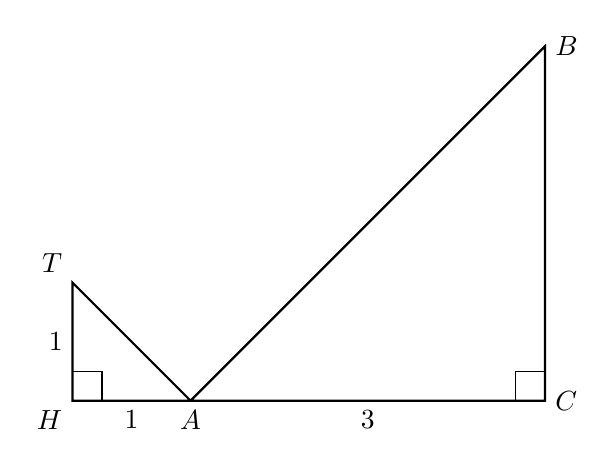
\begin{tikzpicture}[scale=1.5]
          \draw [thick]
          (0,0)node[below]{$A$}--
          (3,0)node[ right]{$C$}--
          (3,3)node[right]{$B$}--cycle;
          \draw (3,0)++(-0.25,0)--++(0,0.25)--+(0.25,0);
          \draw [thick]
          (0,0)--
          (-1,0)node[below left]{$H$}--
          (-1,1)node[above left]{$T$}--cycle;
          \draw (-1,0)++(0.25,0)--++(0,0.25)--+(-0.25,0);
          \node at (1.5,0)[below]{$3$};
          \node at (-0.5,0)[below]{$1$};
          \node at (-1,0.5)[left]{$1$};
        \end{tikzpicture}
    \end{multicols} \vspace{0.75cm}

  \item Using a calculator, find $\theta$ and round to the \emph{nearest whole degree}.
  \begin{enumerate}
    \begin{multicols}{2}
      \item $\theta = \sin^{-1} 0.500$ \vspace{2cm}
      \item $\displaystyle \theta = \cos^{-1} \left(\frac{\sqrt{3}}{2}\right)$
      \item $\tan \theta = 1.000$ \vspace{2cm}
      \item $\displaystyle \cos \theta = 0.707$    \end{multicols}
    \end{enumerate} \vspace{4cm}

\end{enumerate}
\end{document}

